\chapter{Ecologia Comportamental}\label{ch:b3:behavioural-ecology}

Um suricato fica de pé sobre um cupinzeiro enquanto o resto de seu grupo
cava em busca de comida e, quando um gavião aparece, ele late e os outros
disparam para as tocas. A sentinela passou uma hora sem comer e se tornou
o animal mais visível do deserto. Por quê? Um pavão arrasta uma cauda que
lhe custa um quinto de seu orçamento energético e retarda sua fuga dos
tigres. Uma abelha que volta de um campo dança num favo vertical, e o
ângulo de sua dança em relação à vertical é o ângulo da comida em relação
ao sol. Um chapim que caça lagartas num tufo de folhagem o abandona
quando ainda há lagartas a encontrar. Nenhum desses animais leu este
capítulo e, no entanto, cada um se comporta como se tivesse resolvido uma
otimização, um jogo ou um problema de contabilidade de parentesco. A
ecologia comportamental é o estudo do comportamento como um conjunto de
soluções evoluídas: para que serve um comportamento, em termos dos genes
que ele propaga, e quais precisam ser seus custos e benefícios para que a
seleção natural o tenha produzido. Suas ferramentas são as de um
economista --- otimização, \omterm{prop:b3:behavioural-ecology:hawk-dove}{teoria dos jogos}, a contabilidade do
parentesco --- e seu teste é o campo.

\section{Quatro perguntas e a maquinaria do instinto}

\begin{definition}[As perguntas de Tinbergen]\label{def:b3:behavioural-ecology:tinbergen}
\index{quatro perguntas de Tinbergen}\index{padrão fixo de ação}\index{estímulo-sinal}\index{imprinting}\index{período crítico}
Tinbergen (1963) disse que uma explicação completa de qualquer
comportamento precisa responder a quatro perguntas: seu \emph{mecanismo}
(que estímulos e que maquinaria neural o produzem), seu
\emph{desenvolvimento} (como ele surge no indivíduo, a partir de genes e
experiência), sua \emph{função} (como ele contribui para a sobrevivência
e a reprodução) e sua \emph{história evolutiva} (como ele surgiu de um
comportamento ancestral). Os etólogos que as formularam já tinham
estabelecido as duas primeiras. Muitos comportamentos são \emph{padrões
fixos de ação}: sequências estereotipadas disparadas por um simples
\emph{estímulo-sinal} e executadas até o fim uma vez iniciadas --- um
ganso-bravo rola com o bico um ovo deslocado de volta ao ninho e completa
o movimento mesmo que o ovo seja retirado no meio do caminho; um filhote
de gaivota-argêntea bica uma mancha vermelha em qualquer objeto em forma
de bico e bica mais num bastão com três faixas vermelhas que na cabeça de
uma gaivota de verdade; um esgana-gata macho ataca qualquer coisa
vermelha em sua parte inferior, inclusive um furgão do correio visto pela
janela. Outros são aprendidos dentro de uma janela: o \emph{imprinting},
pelo qual um filhote de ganso, em seu primeiro dia, segue e daí em diante
trata como pai o que quer que se mova --- um ganso, Lorenz, uma caixa de
papelão ---, é rápido, irreversível e confinado a um \emph{período
crítico}; o aprendizado do canto nas aves, o exemplo do volume do Ano~2,
tem a mesma forma. A dicotomia entre inato e aprendido é falsa: um
comportamento tem um programa genético que especifica o que deve ser
aprendido, quando e com quem, e o programa é o que evolui.
\end{definition}

\begin{proof}[Evidência]
Os experimentos de campo de Tinbergen fixaram o método. As vespas
cavadoras (\emph{Philanthus}) voltam a um ninho escondido na areia; ele
moveu um anel de pinhas que havia colocado em torno de uma entrada
enquanto a vespa estava fora, e ela procurou no centro do anel deslocado
--- ela havia aprendido os pontos de referência. As gaivotas-de-cabeça-preta
retiram as cascas dos ovos do ninho após a eclosão; ele dispôs ovos ao
lado de cascas pintadas, cascas naturais e outros objetos e contou quais
as gralhas levavam: a superfície interna branca de uma casca atraía os
predadores, e a retirada que parecera asseio era camuflagem. Os
experimentos com filhotes de gaivota quantificaram um \omterm{def:b3:behavioural-ecology:tinbergen}{estímulo-sinal}
oferecendo cabeças de papelão que variavam uma característica de cada
vez. Os gansos que se imprimiram em Lorenz o seguiram a vida toda; patos
imprimidos no primeiro dia numa caixa em movimento não puderam depois ser
levados a seguir um pato.
\end{proof}

\begin{omfigure}
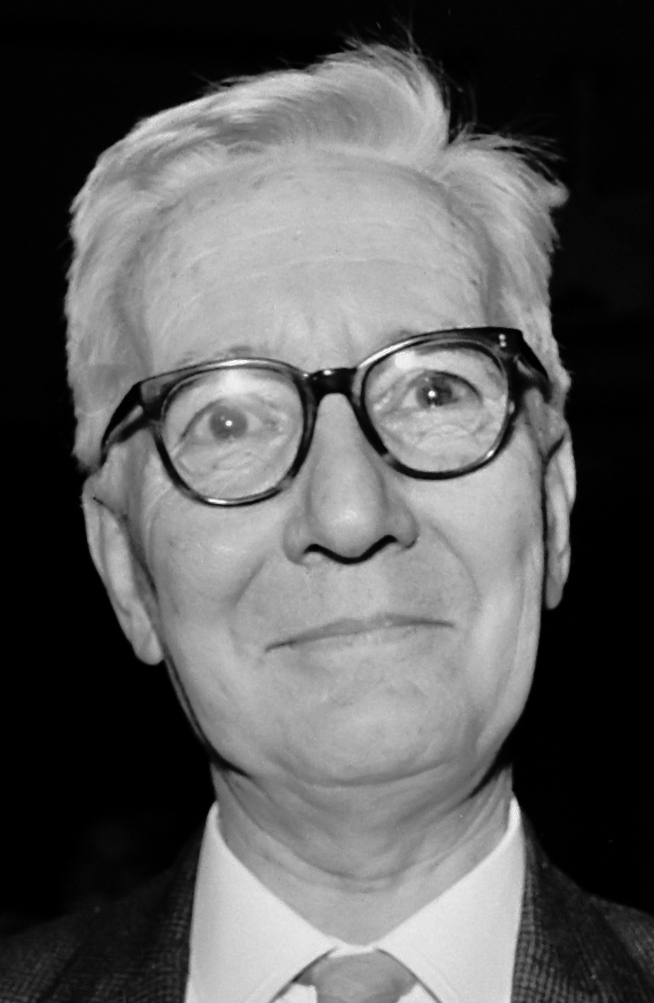
\includegraphics[width=0.36\linewidth]{images/book5/tinbergen.jpg}\hspace{0.04\linewidth}
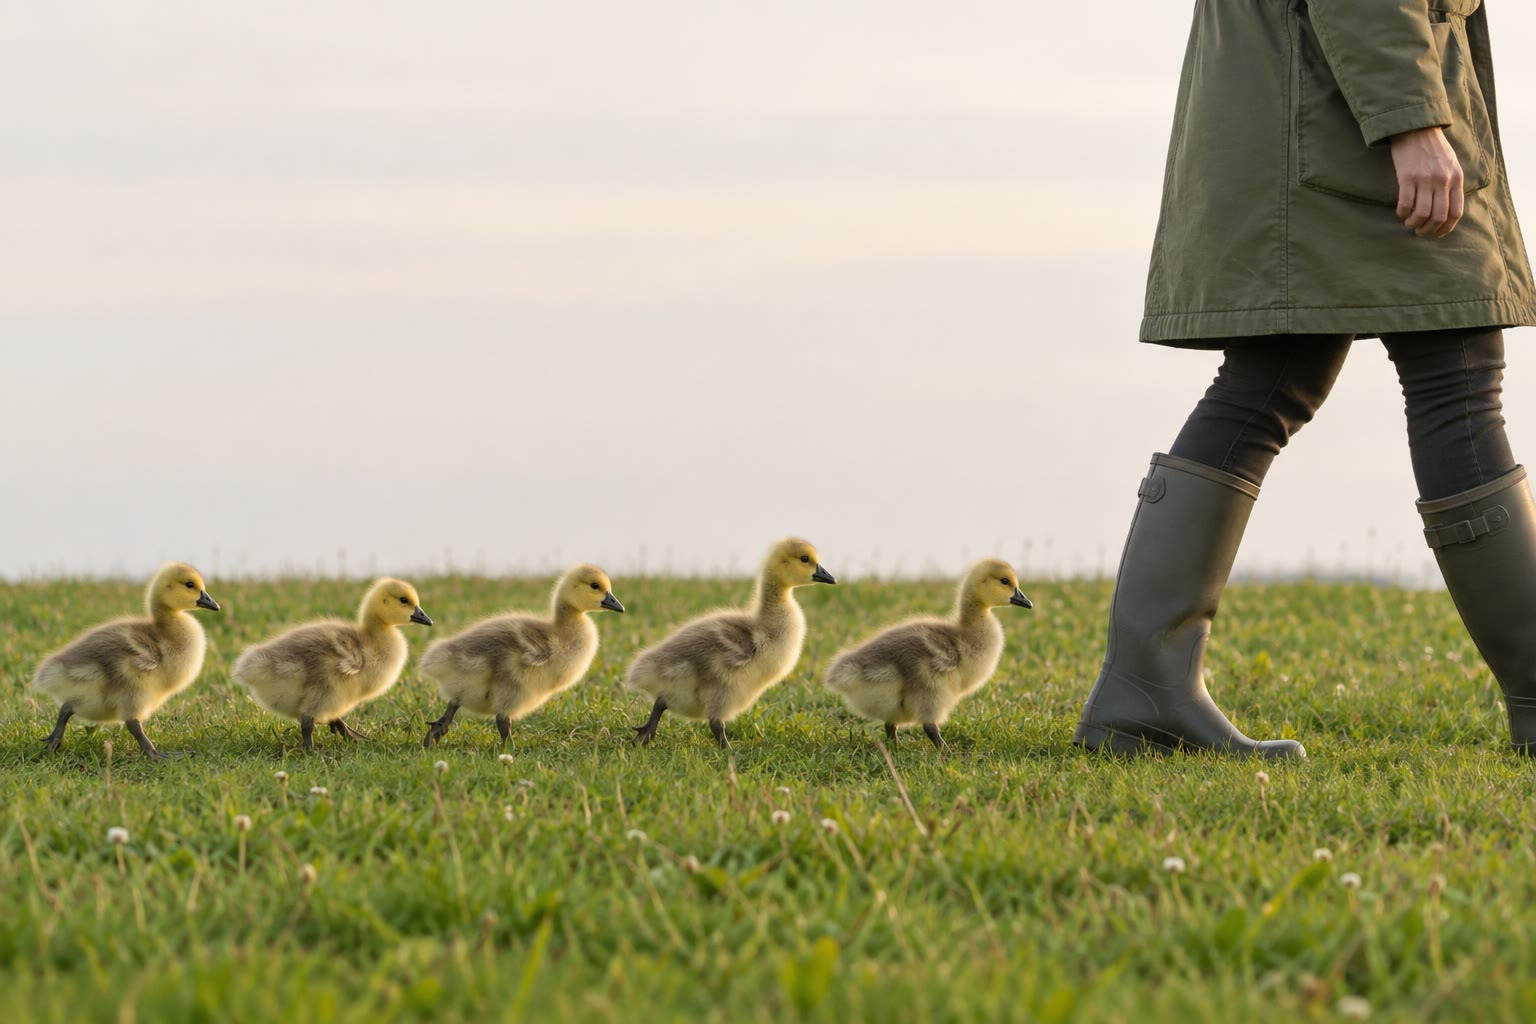
\includegraphics[width=0.52\linewidth]{images/book5/ai/b5-26-goose-imprinting.jpg}

{\small À esquerda: Niko Tinbergen (1907--1988), que levou as perguntas do
comportamento para o campo e as tornou experimentais (fotografia de Rob
Mieremet, Anefo, 1973, CC0). À direita: filhotes de ganso seguindo a
primeira coisa grande em movimento que viram, um dia após a eclosão, e
jamais persuadidos do contrário.}
\end{omfigure}

\section{Decidir: forrageamento ótimo}

\begin{theorem}[O teorema do valor marginal]\label{thm:b3:behavioural-ecology:mvt}
\index{forrageamento ótimo}\index{teorema do valor marginal}\index{tempo de permanência na mancha}\index{moeda}
Um forrageador visita manchas de alimento separadas por um tempo de
viagem $\tau$. Numa mancha ele ganha energia $g(t)$ após um tempo $t$,
com $g$ crescente e côncava (a mancha se esgota). Se ele deixa toda
mancha após um tempo $t$, sua taxa de ganho de longo prazo é $R(t) = g(t)/(\tau + t)$, e o tempo de permanência $t^{*}$ que a maximiza
satisfaz
\[
g'(t^{*}) = \frac{g(t^{*})}{\tau + t^{*}} = R(t^{*}) :
\]
deixe uma mancha quando a taxa instantânea de ganho nela tiver caído à
taxa média de todo o hábitat, viagem incluída (Charnov, 1976).
Consequências: quanto mais longo o tempo de viagem, mais longa a estadia
e mais a fundo cada mancha é esgotada; num hábitat mais rico ($R$ mais
alto) toda mancha é deixada mais cedo e menos esgotada; e todas as
manchas são deixadas na mesma taxa marginal, qualquer que seja sua
qualidade, de modo que uma mancha pobre é deixada quase de imediato e uma
rica só quando já foi trabalhada até a média do hábitat. Para $g(t) = A(1 -
\mathrm{e}^{-t/T_{0}})$ a condição vira $(\tau + t^{*})/T_{0} =
\mathrm{e}^{t^{*}/T_{0}} - 1$, resolvida numericamente: com $\tau = T_{0}$, $t^{*} \approx 1.15\,T_{0}$; com $\tau = 4T_{0}$, $t^{*} \approx
2.0\,T_{0}$.
\end{theorem}
\begin{proof}
$R(t) = g(t)/(\tau + t)$; $R'(t) = [g'(t)(\tau + t) - g(t)]/(\tau +
t)^{2} = 0$ dá $g'(t^{*}) = g(t^{*})/(\tau + t^{*})$. Geometricamente:
trace $g$ contra $t$ com a origem em $-\tau$; $R(t)$ é a inclinação da
reta de $(-\tau, 0)$ a $(t, g(t))$, máxima onde essa reta tangencia a
curva --- que é a condição. Um $\tau$ maior move a origem para a esquerda
e o ponto de tangência para a direita; um hábitat mais rico inclina mais
a tangente e a move para a esquerda. Para a exponencial, $g' = (A/T_{0})
\mathrm{e}^{-t/T_{0}}$ e $g/(\tau + t) = A(1 - \mathrm{e}^{-t/T_{0}})/
(\tau + t)$; igualando e rearranjando obtém-se a equação enunciada e,
substituindo $t^{*} = 1.15T_{0}$ com $\tau = T_{0}$: à esquerda $2.15$, à
direita $\mathrm{e}^{1.15} - 1 = 2.16$.
\end{proof}

\begin{omfigure}
\begin{tikzpicture}
\begin{axis}[
  width=0.68\linewidth, height=5.8cm,
  axis x line=middle, axis y line=left,
  xmin=-4.5, xmax=5, ymin=0, ymax=1.15,
  xlabel={tempo (em unidades de $T_{0}$)}, ylabel={energia ganha na mancha},
  xlabel style={font=\small, at={(axis description cs:0.95,0.0)}, anchor=north}, ylabel style={font=\small},
  tick label style={font=\small}, xtick={-4,-1,0,1.15,2}, xticklabels={$-4T_0$,$-T_0$,0,$1.15$,$2.0$}, ytick={0.5,1}, yticklabels={$0.5A$,$A$},
  clip=false,
]
\addplot[very thick, omDef, domain=0:5, samples=80] {1-exp(-x)};
\draw[thick, omThm] (axis cs:-1,0) -- (axis cs:1.55,1.13);
\draw[thick, omMeth!70!black] (axis cs:-4,0) -- (axis cs:3.5,1.081);
\fill[omThm] (axis cs:1.15,0.6834) circle (2pt); \fill[omMeth!70!black] (axis cs:2,0.8647) circle (2pt);
\draw[dashed, gray] (axis cs:1.15,0) -- (axis cs:1.15,0.6834); \draw[dashed, gray] (axis cs:2,0) -- (axis cs:2,0.8647);
\node[font=\scriptsize, omThm, anchor=north west, align=left] at (axis cs:-4.4,1.1) {viagem curta, $\tau = T_{0}$:\\sair em $t^{*} = 1.15\,T_{0}$,\\mancha \qty{68}{\%} esgotada};
\node[font=\scriptsize, omMeth!70!black, anchor=north west, align=left] at (axis cs:2.4,0.62) {viagem longa, $\tau = 4T_{0}$:\\sair em $t^{*} = 2.0\,T_{0}$,\\\qty{86}{\%} esgotada};
\node[font=\scriptsize, omDef, anchor=north west] at (axis cs:3.0,0.86) {$g(t) = A(1 - \mathrm{e}^{-t/T_{0}})$};
\node[font=\scriptsize, gray, anchor=south] at (axis cs:-2.5,0.02) {viagem};
\end{axis}
\end{tikzpicture}

{\small O teorema do valor marginal desenhado. A curva de ganho se achata
à medida que a mancha se esgota; a reta que vai do início da jornada a um
ponto da curva tem inclinação igual à taxa global de ganho; o melhor
momento de sair é onde essa reta tangencia. Uma jornada mais longa move a
origem para a esquerda e o ponto de tangência para a direita.}
\end{omfigure}

\begin{proof}[Evidência]
Cowie (1977) deixou chapins caçarem larvas escondidas em copos cheios de
serragem num viveiro, com o tempo de viagem entre os copos manipulado por
tampas que demoravam mais ou menos para serem removidas; as aves ficavam
mais tempo em cada copo quando a viagem era mais lenta, acompanhando a
previsão do teorema, e a ultrapassavam ligeiramente na direção que a
contabilidade do custo energético da viagem explica. Os estorninhos que
levavam larvas aos filhotes (Kacelnik, 1984) tomavam cargas maiores de
comedouros colocados mais longe, de novo como exige a solução que
maximiza a taxa para uma curva de carregamento. Nenhum dos dois testes
prova que as aves calculam tangentes; ambos mostram que a seleção
produziu regras práticas cujo resultado está perto do ótimo.
\end{proof}

\section{Disputas: teoria dos jogos}

\begin{proposition}[Falcão--Pomba e a estratégia evolutivamente estável]\label{prop:b3:behavioural-ecology:hawk-dove}
\index{teoria dos jogos}\index{jogo Falcão--Pomba}\index{estratégia evolutivamente estável}\index{seleção dependente da frequência}
Quando o melhor comportamento depende do que os outros fazem, não há
ótimo, apenas um \emph{jogo}. Dois animais disputam um recurso que vale
$V$; um \emph{Falcão} luta até se ferir (custo $C$) ou vencer, e uma
\emph{Pomba} exibe-se e recua se for atacada. Os ganhos médios são
\[
\begin{array}{c|cc}
 & \text{contra Falcão} & \text{contra Pomba}\\ \hline
\text{Falcão} & (V - C)/2 & V\\
\text{Pomba} & 0 & V/2
\end{array}
\]
Uma \emph{\omterm{prop:b3:behavioural-ecology:hawk-dove}{estratégia evolutivamente estável}} (Maynard Smith e Price,
1973) é aquela que, uma vez comum, não pode ser invadida por nenhuma
alternativa rara. Se $V > C$, Falcão é a EEE: lutar compensa mesmo contra
lutadores. Se $V
< C$, nenhuma estratégia pura é estável --- uma
população de Pombas é invadida por Falcões, que vencem toda disputa, e
uma população de Falcões, por Pombas, que evitam as lesões --- e a EEE é
jogar Falcão com probabilidade
\[
p^{*} = \frac{V}{C},
\]
ou, equivalentemente, uma população em que essa fração seja de Falcões.
Na EEE as duas estratégias se saem igualmente bem, cada uma rendendo em
média $V(1 -
V/C)/2$, menos que o $V/2$ que uma população de Pombas
teria partilhado: a disputa custa a todos, e ninguém consegue se sair
melhor sozinho. A seleção aqui é \emph{dependente da frequência}: a
aptidão de uma estratégia cai à medida que ela se torna comum, e é por
isso que as disputas animais são quase sempre exibição e ocasionalmente
guerra, e por que a mistura persiste.
\end{proposition}
\begin{proof}
Seja $p$ a fração que joga Falcão. O ganho esperado de um Falcão é
$W_{H} = p(V
- C)/2 + (1 - p)V$; o de uma Pomba é $W_{D} = (1 - p)V/2$.
$W_{H} - W_{D} =
p(V - C)/2 + (1 - p)V/2 = [V - pC]/2$, positivo para $p < V/C$ e negativo acima disso: os Falcões se espalham quando raros e são
ceifados quando comuns, e a frequência se acomoda onde $W_{H} = W_{D}$,
em $p^{*} = V/C$. A estabilidade decorre da troca de sinal: uma
perturbação de $p$ acima de $p^{*}$ favorece as Pombas e é corrigida;
abaixo, favorece os Falcões. Se $V
\ge C$ a diferença é positiva para
todo $p \le 1$ e Falcão se fixa. O ganho comum em $p^{*}$: $W_{D} = (1 - V/C)V/2$.
\end{proof}

\begin{omfigure}
\begin{tikzpicture}
\begin{axis}[
  width=0.6\linewidth, height=5.4cm,
  axis x line=bottom, axis y line=left,
  xmin=0, xmax=1, ymin=-1, ymax=4.2,
  xlabel={fração de Falcões $p$}, ylabel={ganho esperado},
  xlabel style={font=\small, at={(axis description cs:0.5,-0.12)}, anchor=north}, ylabel style={font=\small},
  tick label style={font=\small}, xtick={0,0.5,1}, xticklabels={0,$p^{*} = V/C$,1}, ytick={0,1,2,4},
  clip=false,
]
\addplot[very thick, omThm, domain=0:1, samples=2] {x*(4-8)/2 + (1-x)*4};
\addplot[very thick, omDef, domain=0:1, samples=2] {(1-x)*4/2};
\draw[dashed, gray] (axis cs:0.5,-1) -- (axis cs:0.5,1);
\fill[black] (axis cs:0.5,1) circle (2pt);
\node[font=\scriptsize, omThm, anchor=north west] at (axis cs:0.5,3.9) {Falcão: $p(V - C)/2 + (1 - p)V$};
\node[font=\scriptsize, omDef, anchor=south west] at (axis cs:0.62,0.9) {Pomba: $(1 - p)V/2$};
\node[font=\scriptsize, anchor=west, align=left] at (axis cs:0.55,2.6) {$V = 4$, $C = 8$:\\EEE em $p^{*} = 0.5$,\\ganho $V(1 - V/C)/2 = 1$};
\draw[->, thick, omThm] (axis cs:0.1,-0.5) -- (axis cs:0.4,-0.5); \draw[->, thick, omDef] (axis cs:0.9,-0.5) -- (axis cs:0.6,-0.5);
\node[font=\tiny, anchor=north] at (axis cs:0.25,-0.55) {Falcões se espalham}; \node[font=\tiny, anchor=north] at (axis cs:0.75,-0.55) {Pombas se espalham};
\end{axis}
\end{tikzpicture}

{\small O \omterm{prop:b3:behavioural-ecology:hawk-dove}{jogo Falcão--Pomba}. Onde as retas de ganho se cruzam, as duas
estratégias se saem igualmente bem e nenhuma consegue se espalhar; de
cada lado, a seleção empurra a frequência de volta. A mistura é estável e
custa a todos, e é com isso que as disputas animais se parecem.}
\end{omfigure}

\begin{example}[Jogos no campo]\label{ex:b3:behavioural-ecology:games}
Os machos da borboleta-malhada-dos-bosques disputam manchas de sol no
chão da floresta: o residente quase sempre vence um breve voo em espiral
e, quando dois machos são enganados de modo que cada um se creia
residente, a luta dura dez vezes mais --- uma convenção (``o residente
vence'') que resolve disputas de modo barato, ela própria uma EEE quando
lutar é caro e o recurso não vale muito. Os machos da mosca-do-esterco
esperam as fêmeas sobre bostas de vaca e vão embora quando a taxa de
chegadas cai ao que uma bosta fresca ofereceria --- o teorema do valor
marginal de novo, num jogo em que o valor da mancha depende de quantos
rivais estão sobre ela. As vespas-dos-figos, os lagartos-de-manchas-laterais
com três tipos de macho que se batem ciclicamente como pedra--papel--tesoura,
e os machos ``furtivos'' do salmão e do peixe-sol, que fecundam ovos
passando rapidamente pelos machos territoriais que não conseguem
enfrentar, são todos misturas mantidas em frequências em que as
alternativas pagam igual. A guerra de desgaste --- dois animais se
exibindo até que um desista, sendo a EEE persistir por um tempo aleatório
tirado de uma distribuição exponencial --- descreve as disputas de
encarada de muitas espécies e prevê, corretamente, que a persistência do
perdedor nada revela sobre quanto tempo ele teria continuado.
\end{example}

\section{Parentes: a regra de Hamilton}

\begin{theorem}[A regra de Hamilton]\label{thm:b3:behavioural-ecology:hamilton}
\index{regra de Hamilton}\index{seleção de parentesco}\index{parentesco}\index{aptidão inclusiva}\index{altruísmo}\index{haplodiploidia}
Um alelo que leva seu portador a realizar um ato que lhe custa $c$
descendentes e dá a um parente $b$ descendentes a mais se espalha se
\[
r\,b > c ,
\]
onde $r$ é o \emph{coeficiente de parentesco}: a probabilidade de que um
gene do receptor seja uma cópia, por descendência, do mesmo gene do
autor --- $1/2$ entre pai e filho ou entre irmãos completos, $1/4$ entre
meios-irmãos, netos, sobrinhos e sobrinhas, e $1/8$ entre primos de
primeiro grau. A grandeza que o alelo maximiza é a \emph{\omterm{thm:b3:behavioural-ecology:hamilton}{aptidão
inclusiva}} de seu portador: sua própria reprodução mais seus efeitos
sobre a reprodução dos parentes, cada um ponderado por $r$. O
\emph{altruísmo} --- comportamento que baixa a reprodução do autor e
eleva a de outro --- evolui, assim, em direção aos parentes, em proporção
ao parentesco, e a regra prevê onde ele deve ser encontrado: nos chamados
de alarme das fêmeas de esquilo-terrestre, que vivem entre suas irmãs e
filhas, e não nos dos machos, que se dispersam; no turno de sentinela dos
suricatos, cujo grupo é uma família; nos auxiliares junto ao ninho das
aves que ajudam seus pais a criar irmãos quando os territórios estão
cheios. Nos himenópteros \emph{haplodiploides} --- machos de ovos não
fecundados, com um só conjunto de cromossomos, e fêmeas com dois --- as
irmãs completas compartilham três quartos de seus genes ($r = 3/4$), mais
do que uma mãe compartilha com suas filhas ($1/2$), o que Hamilton propôs
como razão de as castas estéreis de operárias de formigas, abelhas e
vespas terem surgido ali onze vezes e quase nunca em outros lugares.
\end{theorem}
\begin{proof}
Considere as cópias do alelo. Quando o autor realiza o ato, suas próprias
cópias perdem $c$ em transmissão esperada; o receptor carrega o alelo com
probabilidade $r$ acima da média da população, de modo que o ganho $b$ do
receptor aumenta a transmissão do alelo em $rb$, em média. O alelo
aumenta de frequência quando $rb - c > 0$ (Hamilton, 1964; a dedução
geral, a partir da covariância entre o genótipo de um indivíduo e sua
aptidão, é a equação de Price, aqui admitida). Parentesco: um progenitor
transmite cada gene a um descendente com probabilidade $1/2$; dois irmãos
completos receberam um dado gene do mesmo progenitor com probabilidade
$1/2$, e é a mesma cópia com probabilidade $1/2$, e há dois progenitores:
$r = 2\times\tfrac{1}{2}
\times\tfrac{1}{2} = \tfrac{1}{2}$. Irmãs
haplodiploides: do pai haploide recebem genes idênticos (probabilidade
$1$); da mãe, cópias idênticas com probabilidade $1/2$; fazendo a média
sobre os dois progenitores, $r = (1 + 1/2)/2 = 3/4$.
\end{proof}

\begin{omfigure}
\begin{tikzpicture}[every node/.style={font=\scriptsize}, >=stealth]
  % diploid pedigree
  \node[draw, circle, fill=omDef!30, minimum size=6mm] (m) at (0,3) {}; \node[draw, fill=omDef!30, minimum size=6mm] (f) at (1.6,3) {};
  \node[above, font=\tiny] at (0.8,3.4) {pais diploides};
  \draw[thick] (m) -- (f);
  \node[draw, circle, fill=omThm!40, minimum size=6mm] (a) at (0,1.5) {}; \node[draw, circle, fill=omDef!15, minimum size=6mm] (s) at (1.6,1.5) {};
  \draw[thick] (0.8,3) -- (0.8,2.2) -- (0,2.2) -- (a); \draw[thick] (0.8,2.2) -- (1.6,2.2) -- (s);
  \node[draw, circle, fill=omDef!15, minimum size=6mm] (c) at (1.6,0) {}; \draw[thick] (s) -- (c);
  \node[draw, circle, fill=omDef!15, minimum size=6mm] (o) at (0,0) {}; \draw[thick] (a) -- (o);
  \node[left, omThm, font=\tiny] at (-0.4,1.5) {autor};
  \node[right, font=\tiny] at (1.95,1.5) {irmão completo: $r = 1/2$};
  \node[right, font=\tiny] at (1.95,0) {sobrinha: $r = 1/4$};
  \node[left, font=\tiny] at (-0.4,0) {filho próprio: $1/2$};
  \node[right, font=\tiny] at (1.95,3) {progenitor: $r = 1/2$};
  % haplodiploid
  \begin{scope}[shift={(7.2,0)}]
    \node[draw, circle, fill=omDef!30, minimum size=6mm] (q) at (0,3) {}; \node[draw, fill=omMeth!40, minimum size=6mm] (d) at (1.6,3) {};
    \node[above left, font=\tiny] at (0.1,3.3) {rainha (diploide)}; \node[above right, font=\tiny] at (1.5,3.3) {zangão (haploide)};
    \draw[thick] (q) -- (d);
    \node[draw, circle, fill=omThm!40, minimum size=6mm] (w) at (0,1.5) {}; \node[draw, circle, fill=omDef!15, minimum size=6mm] (w2) at (1.6,1.5) {};
    \draw[thick] (0.8,3) -- (0.8,2.2) -- (0,2.2) -- (w); \draw[thick] (0.8,2.2) -- (1.6,2.2) -- (w2);
    \node[left, omThm, font=\tiny] at (-0.4,1.5) {operária};
    \node[right, align=left, font=\tiny] at (1.95,1.5) {irmã completa: $r = 3/4$\\(genes do pai idênticos,\\os da mãe partilhados com $1/2$)};
    \node[draw, circle, fill=omDef!15, minimum size=6mm] (wd) at (0,0) {}; \draw[thick] (w) -- (wd);
    \node[right, font=\tiny] at (0.35,0) {filha própria: $1/2$ --- menos que uma irmã};
  \end{scope}
  \node[below, align=center] at (4.6,-0.9) {regra de Hamilton: ajude quando $r\,b > c$; uma operária haplodiploide que cria irmãs\\transmite mais de seus genes por descendente que uma que cria filhas};
\end{tikzpicture}

{\small O parentesco em dois tipos de família. Numa genealogia diploide um
irmão vale meio descendente; numa colônia haplodiploide uma irmã vale
mais que uma filha, o que inclina a aritmética para ficar em casa
ajudando.}
\end{omfigure}

\begin{proof}[Evidência]
Sherman (1977) observou esquilos-terrestres de Belding por três verões e
registrou quem dava chamados de alarme quando os predadores se
aproximavam: as fêmeas com parentes por perto chamavam muito mais que as
fêmeas sem parentes, e mais que os machos, que haviam se dispersado de
seu local de nascimento e não tinham parentes ao alcance da voz --- quem
chamava atraía a atenção do predador, e pagava por isso, apenas quando
havia parentes a avisar. Os abelharucos-de-fronte-branca de Emlen ajudam
no ninho em proporção ao parentesco, escolhendo, entre os ninhos
disponíveis, os dos parentes mais próximos. O estudo de longo prazo de
Clutton-Brock sobre suricatos verificou que as sentinelas eram os
indivíduos bem alimentados, que tinham menos a perder, e que a
sobrevivência do grupo --- e, portanto, a dos parentes da sentinela ---
subia com o esforço de sentinela; o custo, porém, mostrou-se menor do que
a história supunha, já que uma sentinela num montículo é muitas vezes a
primeira a alcançar uma toca.
\end{proof}

\begin{omfigure}
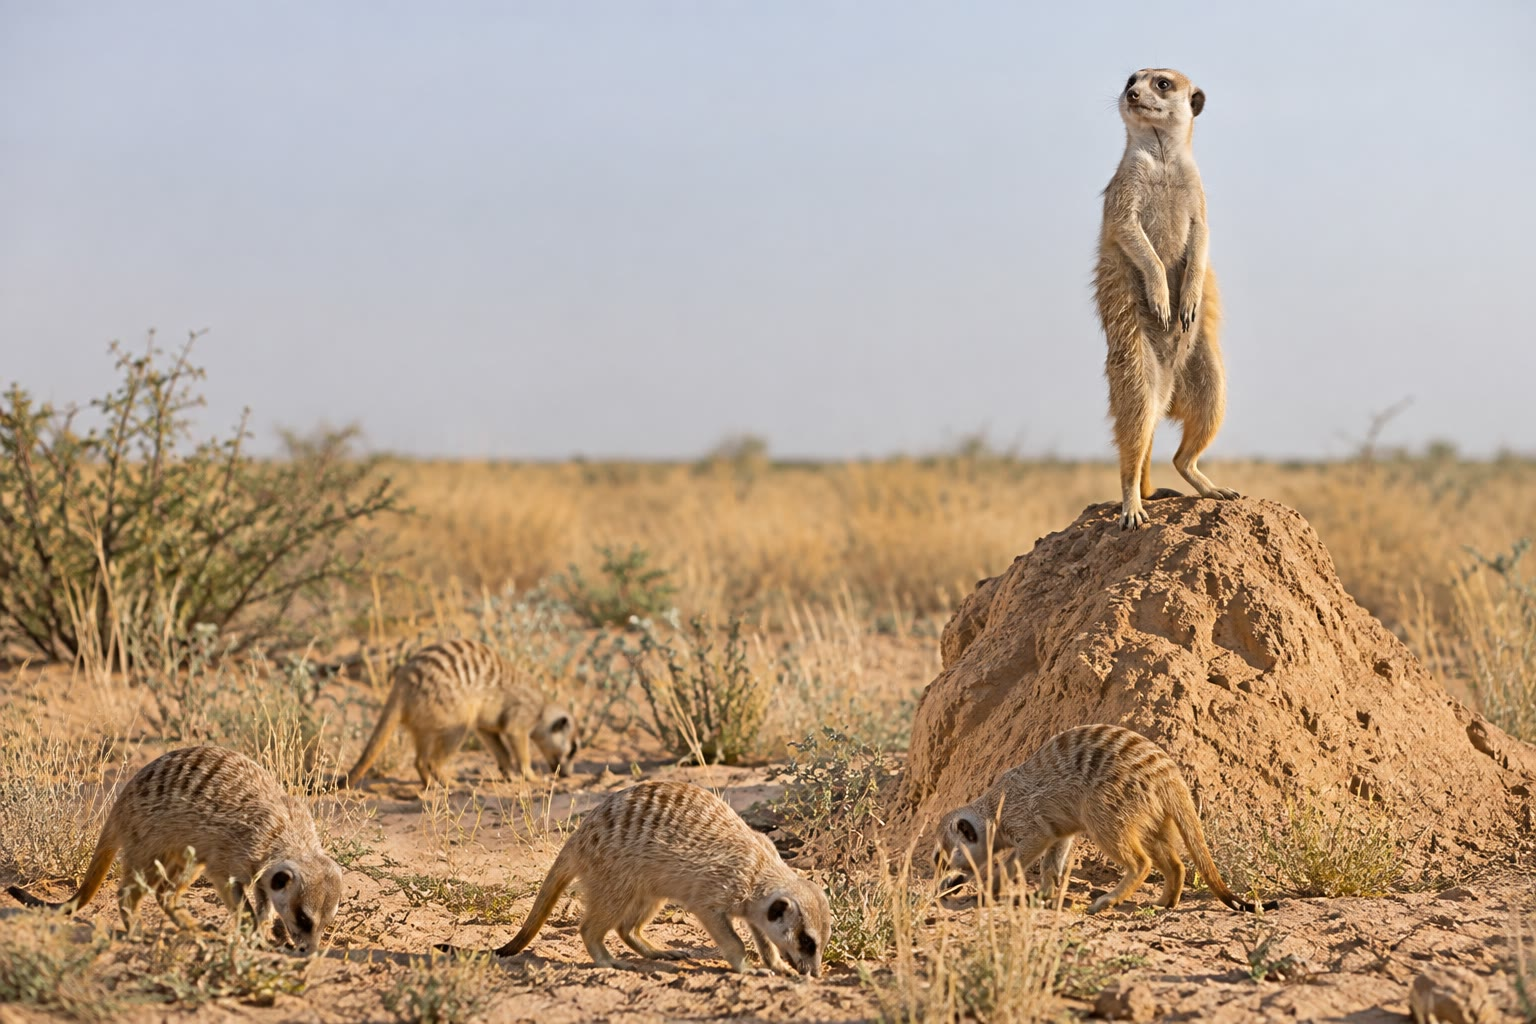
\includegraphics[width=0.46\linewidth]{images/book5/ai/b5-26-meerkat-sentinel.jpg}\hspace{0.04\linewidth}
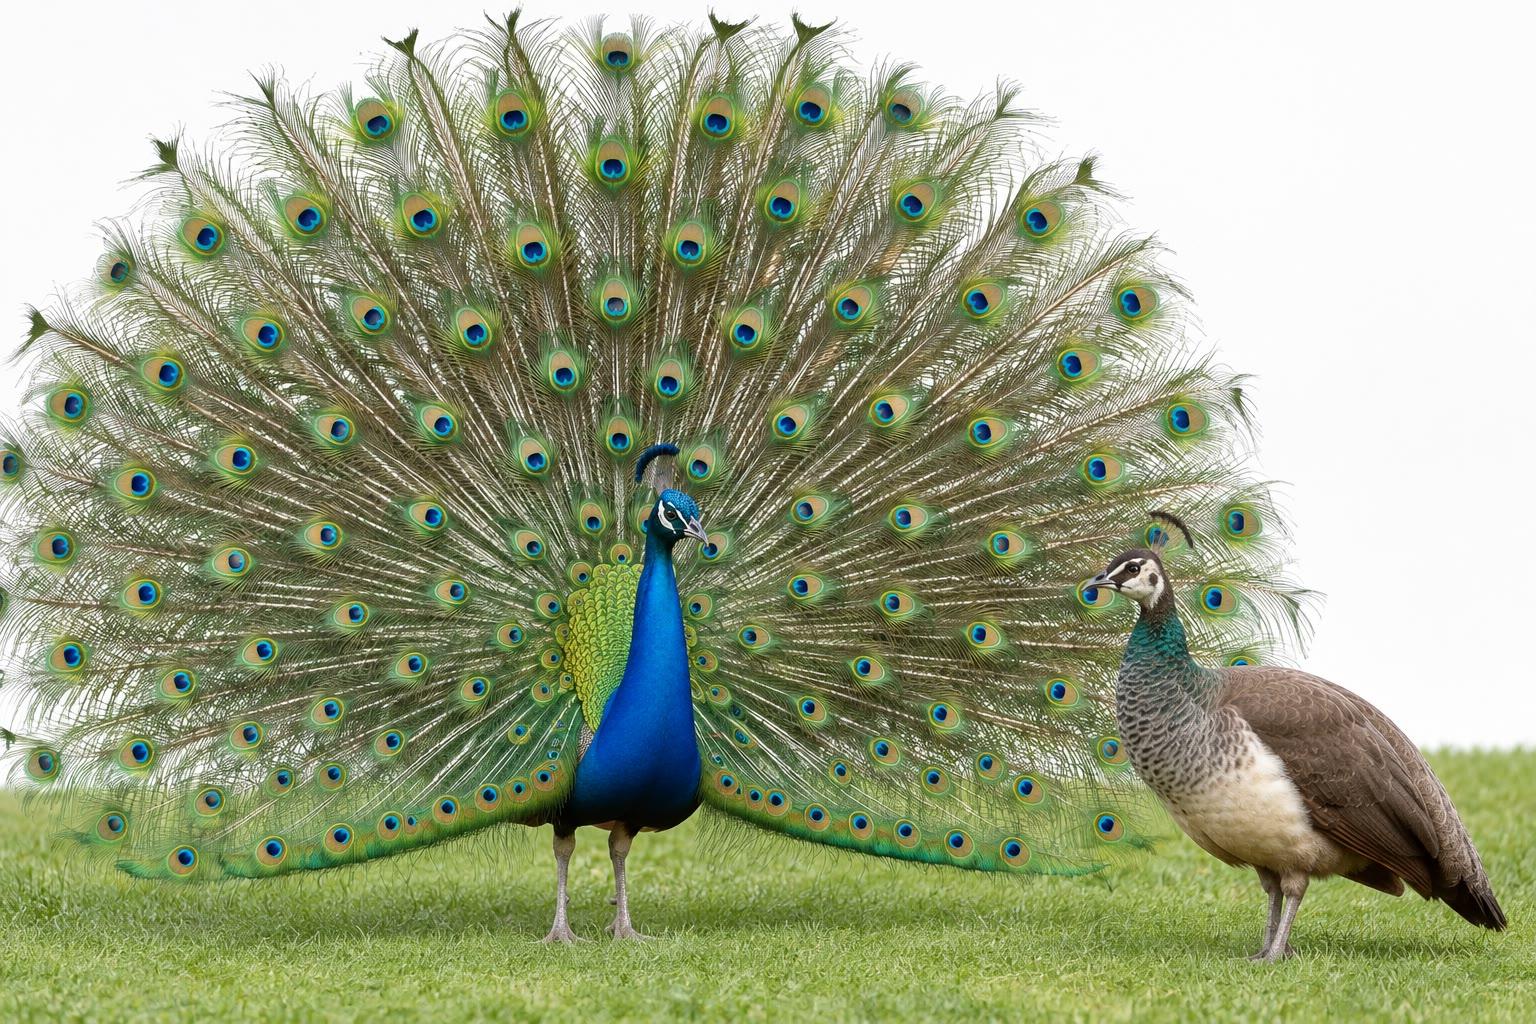
\includegraphics[width=0.46\linewidth]{images/book5/ai/b5-26-peacock-display.jpg}

{\small À esquerda: um suricato em turno de sentinela acima de um grupo de
parentes que forrageia. À direita: um pavão se exibindo para uma pavoa
--- uma estrutura que custa a seu portador em comida e velocidade e nada
lhe compra além da atenção dela.}
\end{omfigure}

\section{Parceiros e mensagens}

\begin{definition}[Seleção sexual]\label{def:b3:behavioural-ecology:sexual-selection}
\index{seleção sexual}\index{gradiente de Bateman}\index{seleção desenfreada}\index{princípio do handicap}\index{bons genes}\index{conflito sexual}
O segundo mecanismo de Darwin: a seleção sobre características que
conquistam parceiros, e não sobrevivência. Sua raiz é a anisogamia --- a
reprodução de uma fêmea é limitada pelos ovos que ela consegue fazer e
prover, e a de um macho, pelas fêmeas que ele consegue fecundar ---, de
modo que na maioria das espécies a aptidão de um macho sobe
acentuadamente com seu número de acasalamentos e a de uma fêmea quase
nada (o \emph{gradiente de Bateman}); os machos então competem pelas
fêmeas e as fêmeas escolhem entre os machos. A competição dá chifres,
galhadas, presas, tamanho grande e as disputas da seção anterior. A
escolha dá ornamentos, e três explicações de por que as fêmeas os
preferem. A \emph{seleção desenfreada} de Fisher: uma preferência por
uma cauda ligeiramente mais longa e a cauda mais longa se espalharam
juntas, cada uma tornando a outra vantajosa, até que o custo da cauda em
sobrevivência equilibrasse seu ganho em acasalamentos. O \emph{handicap}
de Zahavi: um ornamento que só um macho saudável pode se dar ao luxo de
fazer crescer é um \omterm{prop:b3:behavioural-ecology:signals}{sinal honesto} de sua condição, precisamente por ser
caro --- um pavão com a cauda completa tem, comprovadamente, menos
parasitas. \emph{Bons genes} e \emph{benefícios diretos}: a fêmea ganha,
pela herança de seus descendentes ou pelo território e pela comida que o
macho fornece. Os interesses dos dois sexos diferem, e o \emph{conflito
sexual} --- sobre a frequência dos acasalamentos, sobre quem cuida dos
filhotes, sobre o destino do esperma de um parceiro anterior --- é uma
corrida armamentista travada dentro de uma espécie: o líquido seminal
dos machos da mosca-das-frutas encurta a vida da fêmea e eleva sua
postura de ovos, e as fêmeas desenvolvem resistência.
\end{definition}

\begin{proof}[Evidência]
Andersson (1982) cortou e colou as penas da cauda de machos de
viúva-de-cauda-longa no Quênia: os machos com caudas alongadas até o
dobro de seu comprimento natural atraíram quatro vezes mais ninhos novos
a seus territórios que os machos com caudas encurtadas, enquanto os
controles, cujas caudas foram cortadas e recoladas sem alteração, não
foram afetados --- uma preferência feminina por uma cauda mais longa do
que qualquer macho consegue fazer crescer, a assinatura de uma
preferência selecionada para além da característica. Petrie (1994)
verificou que as pavoas acasalavam com os machos cujas caudas tinham mais
ocelos, e que os filhotes desses machos sobreviviam melhor nos bosques
onde eram soltos --- um benefício de \omterm{def:b3:behavioural-ecology:sexual-selection}{bons genes} medido. Bateman (1948)
contou acasalamentos e descendentes de moscas-das-frutas portadoras de
mutações marcadoras e encontrou o gradiente que leva seu nome: o sucesso
reprodutivo dos machos subia linearmente com os acasalamentos, e o das
fêmeas estabilizava depois de um.
\end{proof}

\begin{proposition}[Sinais honestos]\label{prop:b3:behavioural-ecology:signals}
\index{comunicação}\index{sinal honesto}\index{dança do requebrado}\index{sinal referencial}
Um sinal é um ato que muda o comportamento de um receptor e que evoluiu
para isso; ele só é estável se compensar, em média, às duas partes
enviá-lo e responder a ele. Onde as duas têm interesses comuns o sinal
pode ser barato e preciso: a \emph{\omterm{prop:b3:behavioural-ecology:signals}{dança do requebrado}} de uma abelha
forrageira (von Frisch, nos anos 1940) codifica a direção de uma fonte de
alimento como o ângulo da corrida requebrada em relação à vertical --- o
ângulo da fonte em relação ao sol --- e sua distância como a duração da
corrida, cerca de um segundo por quilômetro, e as recrutadas voam até
umas poucas dezenas de metros do alvo; os macacos-vervet dão chamados de
alarme distintos para leopardos, águias e cobras, e os ouvintes respondem
de modo apropriado a cada chamado tocado de um alto-falante escondido ---
sinais \emph{referenciais}. Onde os interesses conflitam, um sinal
precisa ser caro ou impossível de falsificar para continuar honesto ---
o bramido de um veado-vermelho, cuja cadência só um veado em forma
sustenta; o tamanho do coaxar de um sapo, fixado por seu corpo; os
ornamentos do parágrafo anterior ---, ou ele é explorado: os vaga-lumes
de um gênero imitam os lampejos das fêmeas de outro para comer os machos
que vêm, e a súplica dos filhotes de cuco supera a dos próprios filhotes
do hospedeiro. A teoria da sinalização prevê, assim, a forma de um sinal
a partir da relação entre as partes: barato e informativo entre parentes
e parceiros cujos interesses coincidem, caro e ritualizado entre rivais,
e uma corrida armamentista entre predador e presa.
\end{proposition}
\admitted

\begin{omfigure}
\begin{tikzpicture}[every node/.style={font=\scriptsize}, >=stealth]
  % field view
  \node[above] at (0,3.2) {no campo};
  \draw[->, thick, gray] (0,0) -- (0,2.6) node[above, font=\tiny] {rumo ao sol};
  \fill[omDef!60] (0,0) circle (0.12); \node[below, font=\tiny] at (0,-0.2) {colmeia};
  \draw[->, very thick, omThm] (0,0) -- ({2.4*sin(40)},{2.4*cos(40)}); \node[right, font=\tiny, omThm] at ({2.4*sin(40)},{2.4*cos(40)}) {comida, \qty{1}{km}};
  \draw[omThm] (0,1.0) arc[start angle=90, end angle=50, radius=1.0]; \node[font=\tiny, omThm] at (0.55,1.25) {$40^{\circ}$};
  % comb view
  \begin{scope}[shift={(6.2,0)}]
    \node[above] at (0,3.2) {no favo vertical};
    \draw[very thick, gray!60] (-1.8,-0.4) rectangle (1.8,3.0);
    \draw[->, thick, gray] (0,0) -- (0,2.6) node[above, font=\tiny] {para cima (= sol)};
    \draw[->, very thick, omThm] (0,0) -- ({1.6*sin(40)},{1.6*cos(40)}); \node[below, align=center, font=\tiny, omThm] at (0,-0.5) {corrida requebrada: $40^{\circ}$ da vertical;\\duração $\approx \qty{1}{s}$ por km};
    \draw[omThm, dashed] ({1.6*sin(40)},{1.6*cos(40)}) .. controls (1.3,0.4) and (0.5,-0.3) .. (0,0);
    \draw[omThm, dashed] ({1.6*sin(40)},{1.6*cos(40)}) .. controls (-0.2,1.2) and (-0.6,0.3) .. (0,0);
    \draw[omThm] (0,0.8) arc[start angle=90, end angle=50, radius=0.8]; \node[font=\tiny, omThm] at (0.45,1.0) {$40^{\circ}$};
  \end{scope}
  \node[right, align=left] at (9.2,1.3) {um código simbólico: a gravidade\\representa o sol, e o tempo,\\a distância; as recrutadas chegam\\a dezenas de metros};
\end{tikzpicture}

{\small A \omterm{prop:b3:behavioural-ecology:signals}{dança do requebrado}. O ângulo da corrida em relação à vertical é
o ângulo da comida em relação ao sol; o comprimento da corrida é a
distância. Um sinal tão barato e tão preciso é possível porque a
dançarina e sua plateia são irmãs com o mesmo interesse.}
\end{omfigure}

\begin{omfigure}
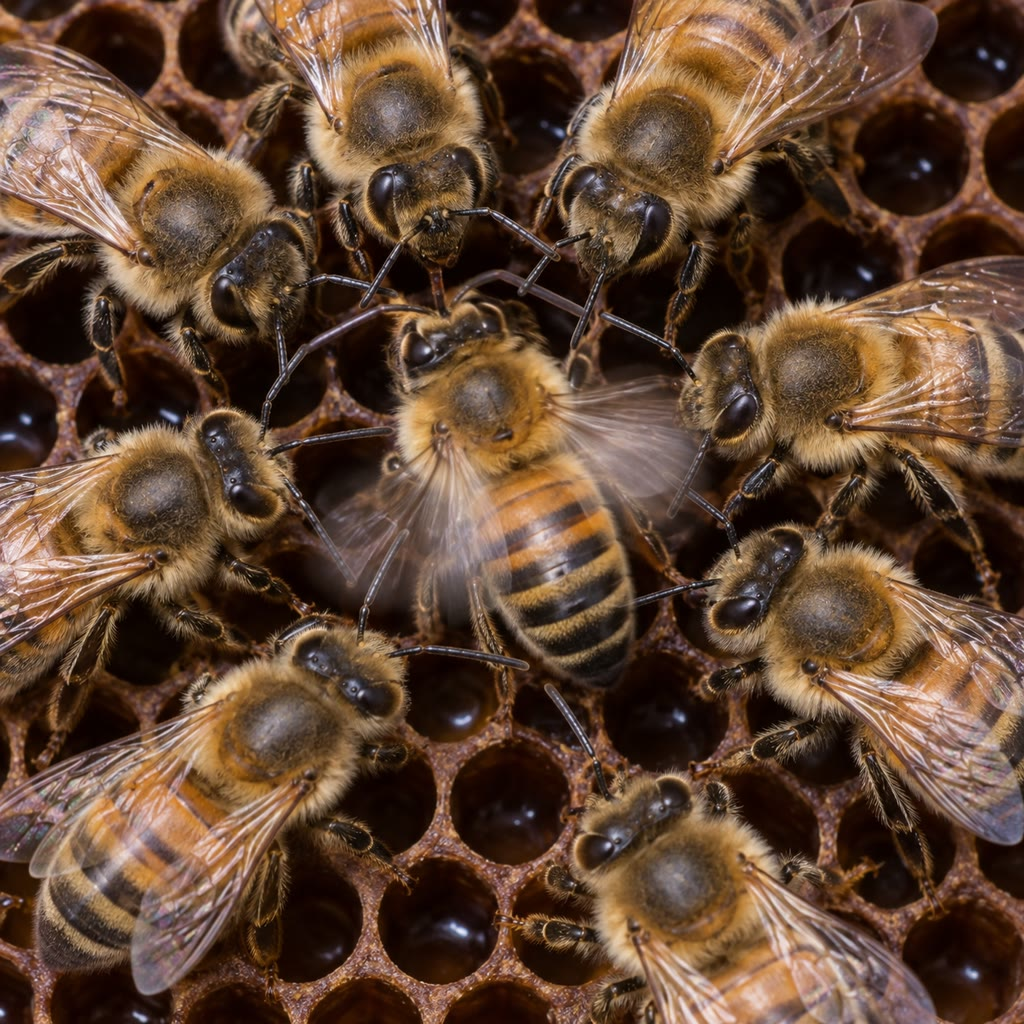
\includegraphics[width=0.4\linewidth]{images/book5/ai/b5-26-bee-dance.jpg}

{\small Uma forrageira dançando no favo, rodeada por operárias que leem o
ângulo e o ritmo de sua corrida.}
\end{omfigure}

\begin{remark}[Por que os animais parecem calcular]\label{rem:b3:behavioural-ecology:remark}
O chapim não deriva $g(t)/(\tau + t)$, o suricato não calcula $r$ e a
pavoa nunca ouviu falar de handicap. Cada um carrega regras --- sair
quando as capturas ficam raras, chamar quando o grupo é família,
preferir o mais vistoso --- que a seleção moldou porque os animais que as
seguiam deixavam mais descendentes; a matemática é nossa, um modo de
perguntar o que as regras precisam alcançar para que isso seja assim, e
de prever comportamentos em situações que os animais nunca encontraram.
Quando as previsões falham --- o chapim fica tempo demais, o custo da
sentinela é menor que o suposto ---, a falha é informativa: uma moeda
estava errada, uma restrição foi esquecida, um parente foi mal contado. O
assunto é uma conversa, década após década, entre um caderno de campo e
uma linha de álgebra, e as quatro perguntas que Tinbergen formulou
continuam sendo o quadro para os dois.
\end{remark}

\section{Exercícios}

\begin{exercise}[$\star$]\label{exo:b3:behavioural-ecology:1}
Enuncie as \omterm{def:b3:behavioural-ecology:tinbergen}{quatro perguntas de Tinbergen} e responda a cada uma, numa
frase, para a \omterm{prop:b3:behavioural-ecology:signals}{dança do requebrado}.
\end{exercise}

\begin{exercise}[$\star$]\label{exo:b3:behavioural-ecology:2}
O que é um \omterm{def:b3:behavioural-ecology:tinbergen}{padrão fixo de ação} e um \omterm{def:b3:behavioural-ecology:tinbergen}{estímulo-sinal}? Dê dois exemplos e
explique o que o bastão ``supranormal'' com três faixas vermelhas
mostrou.
\end{exercise}

\begin{exercise}[$\star$]\label{exo:b3:behavioural-ecology:3}
Em palavras, o que diz o teorema do valor marginal, e o que ele prevê
sobre o uso das manchas quando o tempo de viagem dobra?
\end{exercise}

\begin{exercise}[$\star$]\label{exo:b3:behavioural-ecology:4}
Defina uma EEE. Por que uma população de Pombas puras não é uma EEE, e
por que a mistura Falcão--Pomba custa a todos?
\end{exercise}

\begin{exercise}[$\star\star$]\label{exo:b3:behavioural-ecology:5}
Falcão--Pomba com $V = 6$, $C = 10$: calcule $p^{*}$, o ganho de cada
estratégia na EEE e o ganho que uma população só de Pombas teria. Repita
para $V = 12$, $C = 10$.
\end{exercise}

\begin{exercise}[$\star\star$]\label{exo:b3:behavioural-ecology:6}
Uma função de ganho $g(t) = A(1 - \mathrm{e}^{-t/T_{0}})$ com $T_{0} =
\qty{2}{min}$. Encontre $t^{*}$ para $\tau = 2$ e $\tau = 8$ minutos (use
os valores do capítulo), a fração de cada mancha consumida e a taxa de
longo prazo $R$ como fração de $A$ por minuto.
\end{exercise}

\begin{exercise}[$\star\star$]\label{exo:b3:behavioural-ecology:7}
Calcule $r$ entre: meios-irmãos; avô e neto; primos de primeiro grau; uma
operária haplodiploide e seu irmão; uma rainha haplodiploide e seu filho.
Explique os dois últimos.
\end{exercise}

\begin{exercise}[$\star\star$]\label{exo:b3:behavioural-ecology:8}
Um chamado de alarme custa a quem chama uma chance de \qty{2}{\%} de
morte e salva cada um de $n$ parentes próximos de uma chance de
\qty{1}{\%}. Para que $n$ a regra de Hamilton favorece chamar, se os
parentes forem irmãos completos? E se forem sobrinhos? E se não forem
aparentados?
\end{exercise}

\begin{exercise}[$\star\star$]\label{exo:b3:behavioural-ecology:9}
A cauda de uma viúva-de-cauda-longa tem \qty{50}{cm}; alongada a
\qty{75}{cm}, ela atrai o dobro de ninhos; encurtada a \qty{25}{cm}, a
metade. Se a sobrevivência cai \qty{20}{\%} a cada \qty{25}{cm}
acrescentados, que cauda maximiza o produto de acasalamentos e
sobrevivência, e por que a cauda natural poderia ser mais curta que essa?
\end{exercise}

\begin{exercise}[$\star\star\star$]\label{exo:b3:behavioural-ecology:10}
Acrescente uma terceira estratégia, Retaliadora, que se exibe como uma
Pomba mas revida se for atacada. Escreva seus ganhos contra Falcão, Pomba
e ela mesma (contra Falcão ela luta: $(V - C)/2$; contra Pomba e
Retaliadora ela reparte: $V/2$). Mostre que uma população de
Retaliadoras não pode ser invadida por Falcões quando $V < C$, e discuta
se Pombas podem entrar por deriva.
\end{exercise}

\begin{exercise}[$\star\star\star$]\label{exo:b3:behavioural-ecology:11}
Numa guerra de desgaste, cada contendor persiste por um tempo tirado de
uma distribuição; a EEE é exponencial com média $V/$(custo por unidade de
tempo). Explique por que um tempo fixo de persistência não pode ser uma
EEE, e por que uma distribuição exponencial torna a persistência futura
esperada de um oponente ainda em exibição independente de quanto tempo
ele já se exibiu.
\end{exercise}

\begin{exercise}[$\star\star\star$]\label{exo:b3:behavioural-ecology:12}
O argumento de Hamilton para a haplodiploidia prevê que as operárias
deveriam preferir criar irmãs ($r = 3/4$) a irmãos ($r = 1/4$), enquanto
a rainha valoriza filhos e filhas igualmente. Preveja a razão sexual dos
reprodutores que uma colônia deveria produzir se as operárias a
controlarem, e se a rainha a controlar; diga o que Trivers e Hare
encontraram e o que uma rainha que acasala com vários machos faz ao
argumento.
\end{exercise}

\section{Problema: A Aritmética da Sentinela}

\begin{problem}[{Problema de fim de semana --- um dia num grupo de
suricatos feito como ecologia comportamental: os tempos de mancha do
teorema do valor marginal, as disputas do jogo Falcão--Pomba e sua EEE, a
contabilidade de parentesco do turno de sentinela e de uma colmeia
haplodiploide, e o custo de um ornamento, terminando no tempo de
permanência na mancha, na frequência de Falcões e no limiar de Hamilton
da sentinela}]
\label{pb:b3:behavioural-ecology:1}
Dados: manchas de forrageio com $g(t) = A(1 - \mathrm{e}^{-t/T_{0}})$,
$T_{0}
= \qty{3}{min}$, $A = \qty{60}{kJ}$; viagem entre manchas $\tau =
\qty{3}{min}$ (hábitat denso) ou \qty{12}{min} (esparso). Disputas por
uma toca: $V = 10$, $C = 30$ (unidades de aptidão). Sentinela: uma hora
de turno custa à sentinela $c = 0.03$ equivalentes-descendentes
(alimentação perdida, exposição); ela reduz o risco de predação de cada
companheiro de grupo, o que vale $b = 0.01$ equivalente-descendente para
cada um; o grupo tem $n$ membros com parentesco médio $\bar r$. Colmeia:
uma operária pode criar $k$ irmãs ou $k$ filhas próprias com o mesmo
esforço. Ornamento: um comprimento de cauda $L$ dá acasalamentos $m(L) = L/20$ e sobrevivência $s(L) = 1 - (L/100)^{2}$, com $L$ em cm.

\medskip
\noindent\textbf{Parte I --- Manchas.}
\begin{enumerate}
  \item Escreva a taxa de longo prazo $R(t)$ e a condição de valor
        marginal para este $g$.
  \item Mostre que a condição se reduz a $(\tau + t)/T_{0} = \mathrm{e}^{t/T_{0}}
        - 1$, e resolva-a para $\tau = T_{0}$ (tente
        $t = 1.15\,T_{0}$).
  \item Resolva para $\tau = 4T_{0}$ (tente $t = 2.0\,T_{0}$).
  \item Para cada caso: tempo de permanência em minutos, energia por
        mancha, fração da mancha consumida e taxa $R$ em kJ/min.
  \item Uma regra prática: ``sair depois de \qty{5}{min} fixos.''
        Calcule $R$ para os dois hábitats e compare com o ótimo. A regra
        é boa o bastante?
  \item Outra regra: ``sair quando passarem \qty{20}{s} sem uma
        captura.'' Explique por que essa regra do tempo de desistência
        aproxima o teorema, e em que direção ela falha quando as manchas
        diferem em riqueza.
\end{enumerate}

\medskip
\noindent\textbf{Parte II --- Disputas.}
\begin{enumerate}[resume]
  \item Escreva a matriz de ganhos e calcule $p^{*}$.
  \item Ganho de Falcão e de Pomba quando $p = 0.1$, $p = p^{*}$ e $p =
        0.6$; que estratégia se espalha em cada caso?
  \item Ganho na EEE; compare com o ganho de uma população só de Pombas.
        Quanto a população perde por disputa em razão da possibilidade de
        lutar?
  \item Uma seca eleva $V$ a $40$ (tocas escassas). Nova EEE? O que isso
        prevê sobre as lutas em anos difíceis?
  \item Burguesa: ``Falcão se residente, Pomba se invasora'', cada papel
        metade do tempo. Seu ganho contra si mesma é $V/2$, sem lutas.
        Mostre que os Falcões não conseguem invadir uma população Burguesa
        quando $V
        < C$, e explique a borboleta-malhada-dos-bosques.
  \item Explique numa frase por que é a dependência da frequência, e não
        um ótimo, que governa esse comportamento.
\end{enumerate}

\medskip
\noindent\textbf{Parte III --- Parentes.}
\begin{enumerate}[resume]
  \item A regra de Hamilton para a sentinela: condição sobre $n\bar r$.
        Para que $n\bar r$ o turno compensa?
  \item Um grupo de $n = 8$ irmãos completos ($\bar r = 1/2$): compensa?
        Um grupo de 8 animais não aparentados? Um grupo de 8
        meios-irmãos?
  \item A sentinela está bem alimentada, de modo que seu $c$ cai a
        $0.01$. Limiar agora? Por que isso prevê que as sentinelas são os
        indivíduos bem alimentados?
  \item A colmeia: valor em \omterm{thm:b3:behavioural-ecology:hamilton}{aptidão inclusiva} de $k$ irmãs contra $k$
        filhas. Qual uma operária deveria preferir, e em que proporção?
  \item A rainha acasalou com três machos igualmente: parentesco médio
        das operárias com as irmãs? A preferência sobrevive?
  \item Explique por que a regra de Hamilton não exige que o autor
        reconheça parentes, e que regra prática um esquilo-terrestre
        poderia de fato usar.
\end{enumerate}

\medskip
\noindent\textbf{Parte IV --- Ornamentos.}
\begin{enumerate}[resume]
  \item Aptidão $W(L) = m(L)\,s(L)$. Calcule $W$ para $L = 20$, $40$,
        $60$, $80$.
  \item Encontre analiticamente o $L$ que maximiza $W$, e o $W$ ali.
  \item O custo em sobrevivência fica mais íngreme, $s = 1 - (L/70)^{2}$
        (chega um predador). Novo ótimo? Em que direção, e por que isso
        prevê que a cauda evolui acompanhando a predação?
  \item O experimento de Andersson dobrou as caudas para \qty{75}{cm} e
        dobrou os ninhos. A preferência feminina por caudas mais longas
        ``além do ótimo'' é consistente com a explicação da \omterm{def:b3:behavioural-ecology:sexual-selection}{seleção
        desenfreada}, com a do handicap, ou com as duas?
  \item Por que um ornamento barato não é um \omterm{prop:b3:behavioural-ecology:signals}{sinal honesto}, e como o
        custo da questão~21 o torna honesto?
  \item \omterm{def:b3:behavioural-ecology:sexual-selection}{Gradientes de Bateman}: os machos ganham $0.8$ descendente por
        acasalamento extra, e as fêmeas, $0.1$. Explique num parágrafo
        como essa assimetria gera tanto as disputas da Parte~II quanto os
        ornamentos da Parte~IV.
  \item Resuma: $t^{*}$ no hábitat denso (questão~4), $p^{*}$
        (questão~7) e o limiar $n\bar r$ da sentinela (questão~13).
\end{enumerate}
\end{problem}
